\section{Implementation Details}
\label{SEC:Implementation}

\begin{figure*}[t]
  \center{}
  \fbox{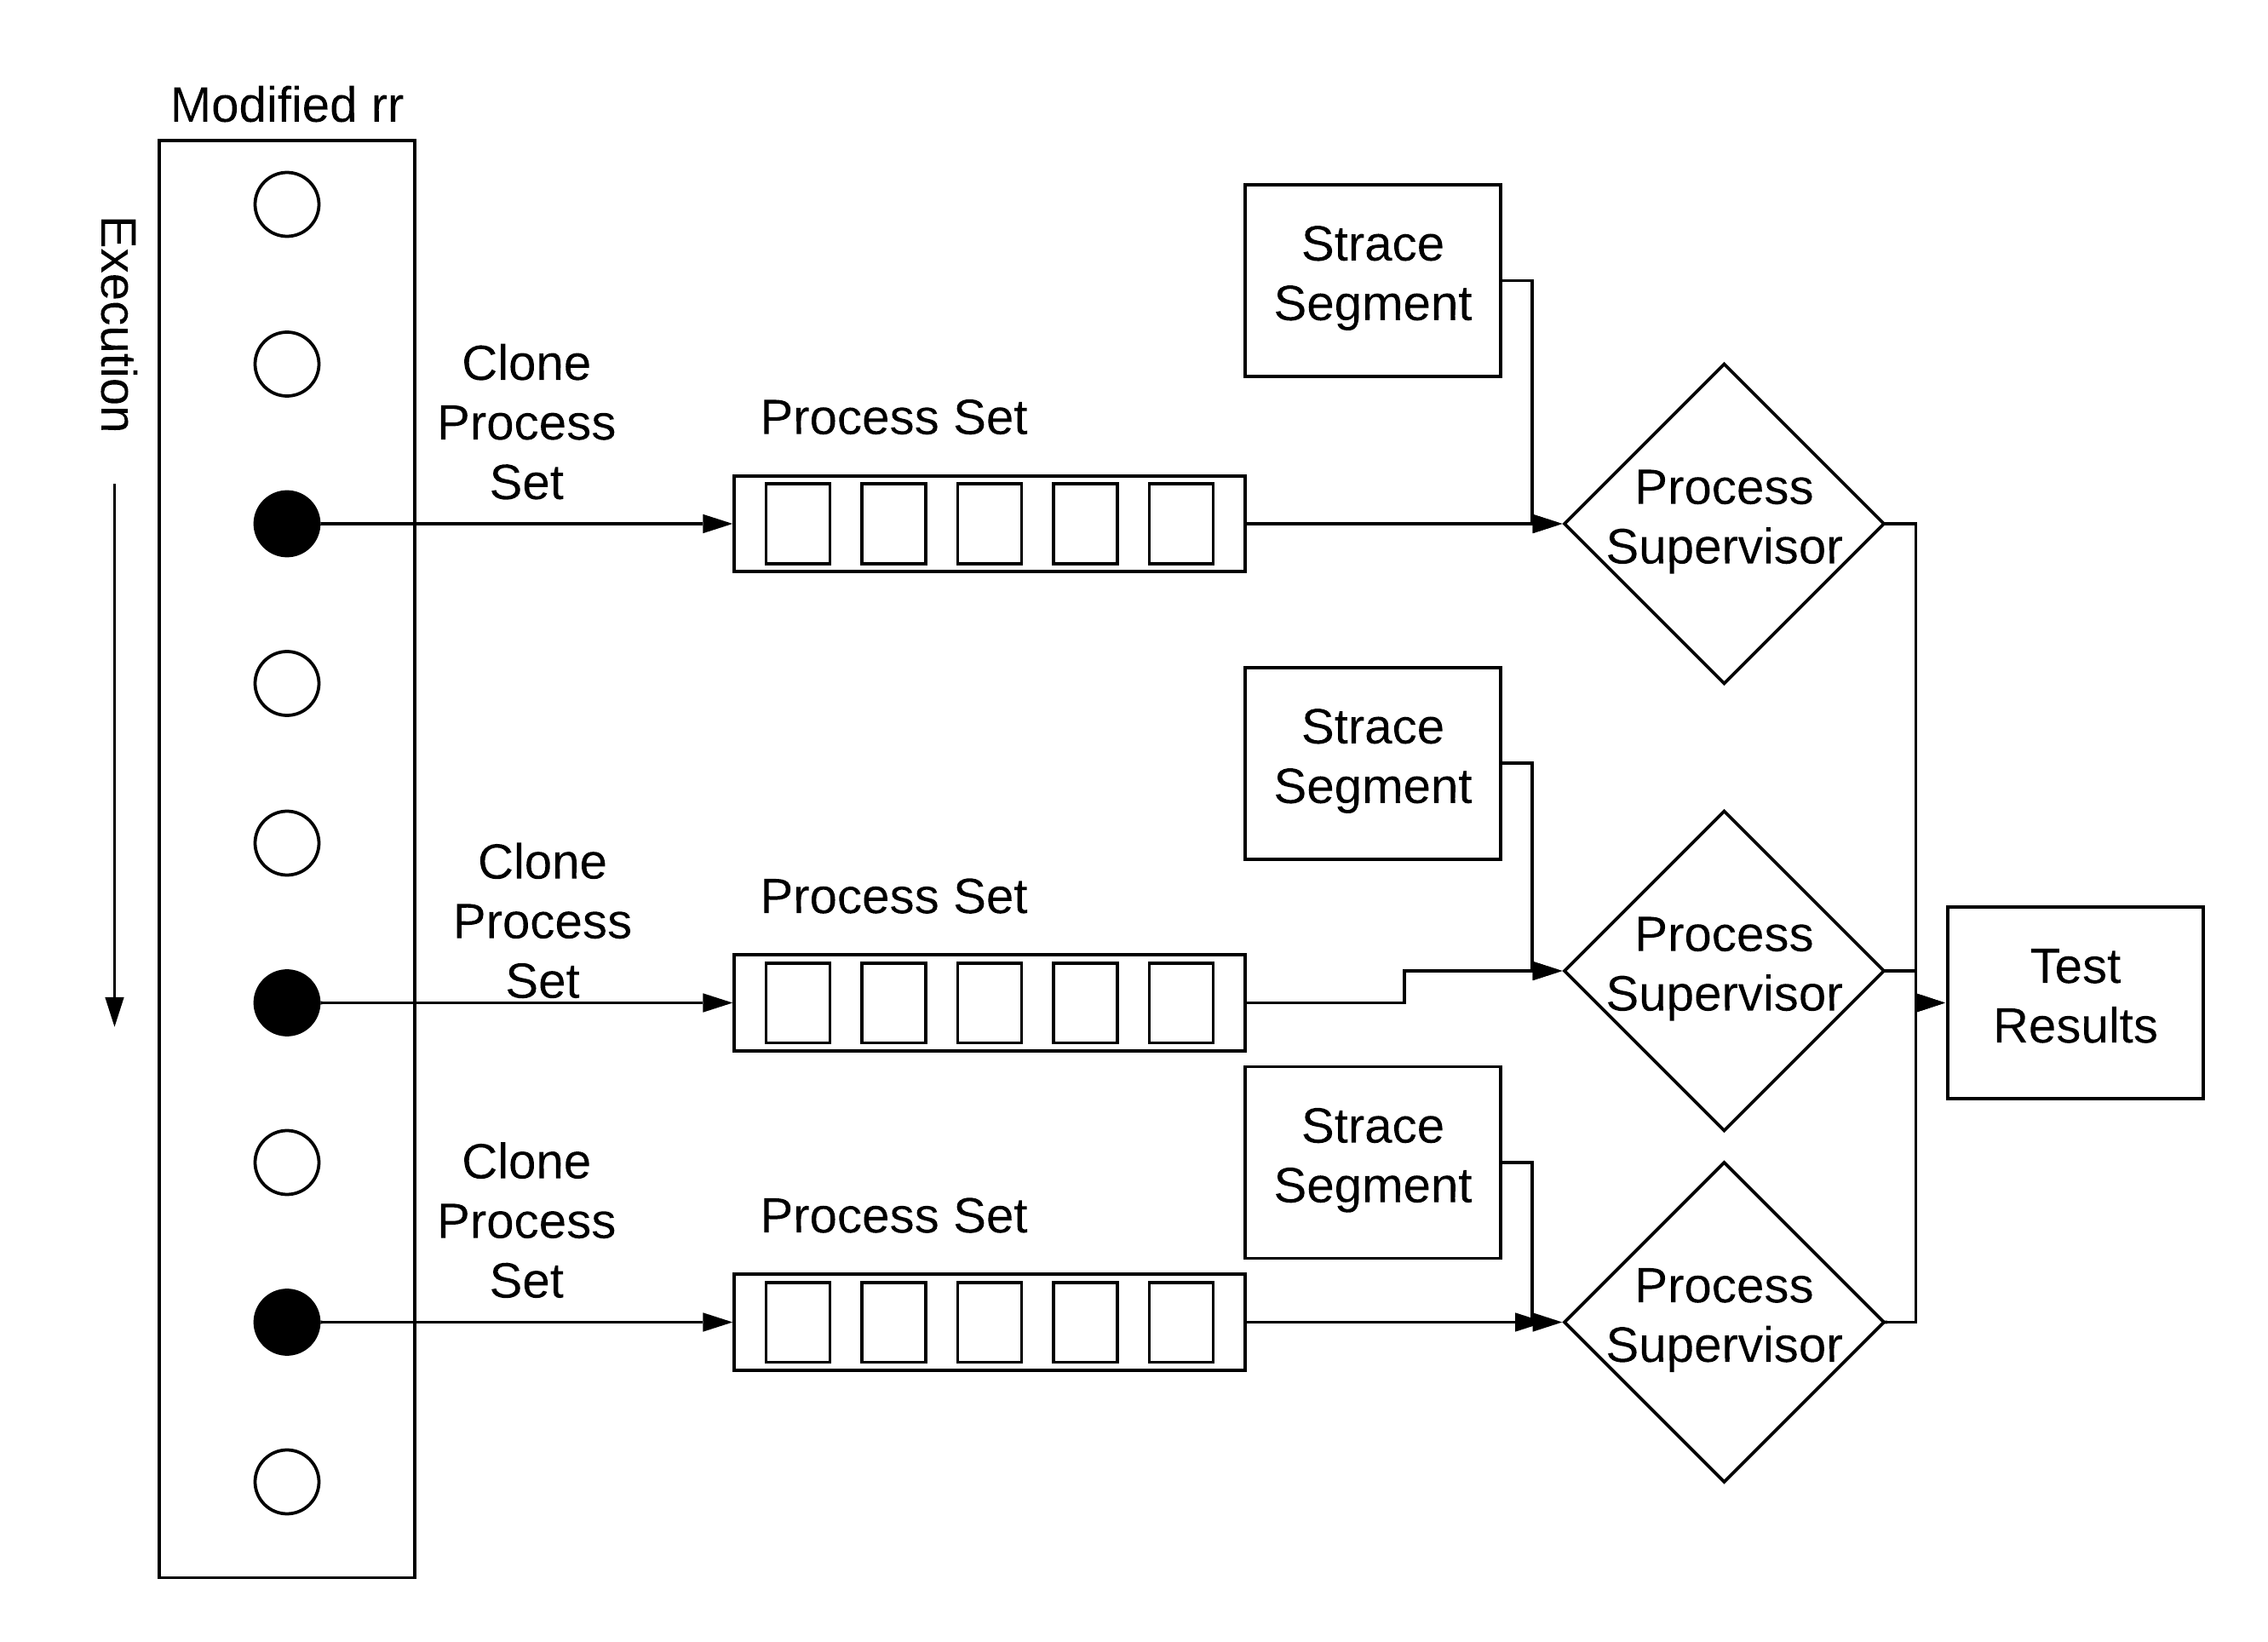
\includegraphics[scale=.65]{images/architecture}}
  \caption{Diagram illustrating CrashSimulator's Architecture.  During the
    course of a single rr execution, clone process sets are generated at
    specific rr events.  A CrashSimlator supervisor process attaches to
    these process sets and uses a strace-style system call listing to feed
    subsequent system call activity and inject unusual environmental
    conditions.}
  \label{figure:architecture}
\end{figure*}

As can be seen in Figure~\ref{figure:architecture},
our implementation of CrashSimulator uses a combination of a modified
version of {\tt rr}, a
record-and-replay debugger, and our own process supervisor
to accomplish the above.  This arrangement arose as a result of several
phases of prototyping that revealed weaknesses in more naive strategies.
Early work on an initial prototype revealed relaunching an
application and associated machinery for each test could result in
poor performance.  One of the goals of our current prototype
was so rectify this situation by eliminating as much unnecessary execution
as possible.  We achieved this by introducing a dramatic amount of
parallelism into CrashSimulator's testing process.
Central to achieving this end is the technique of
{\tt process set cloning}.  The idea behind this technique
is to generate copies
of an application's processes at specific points in execution and conduct
tests on these clones rather than the original processes.  This allows the
original processes to continue execution alleviating the need to restart
the application for each test.  This allows subsequent tests
to avoid wasting effort executing portions of the application preceding
the test.

In CrashSimulator, we implemented this technique by extending the
capabilities of the {\tt rr} record and replay debugger.  {\tt rr} manages
the full set of processes an application requires and offers the ability to
make a copy of it so that users can test debugging
hypotheses without damaging the originals.  Our modified version of {\tt
rr} extends this capability to allow process sets to be liberated from {\tt
rr} so that we can perform CrashSimulator's tests on them.
This means that we can rely on {\tt rr}
to store the information necessary to perform the bulk of
replay that must take place before the application reaches the point in
execution where testing will be performed.  When this point is reached we
take advantage of these combined capabilities
to create a
copy of the set of processes being replayed and liberate them so our
CrashSimulator process supervisor can take over replay responsibilities.

Process sets generated by {\tt rr} are created in a stopped state and
remain until they are attached to and utilized by a CrashSimulator
supervisor.  Each process set has its own supervisor process to inject
its configured environmental anomaly.  The
supervisor wakes up the process set it is managing and simulates any
subsequent system calls it makes.  The data necessary for this
simulation is
supplied as a system call listing formatted after the style of {\tt strace}
output, that describes the results and side effects for each system
call. The output is engineered in such a way to contain the
elements required to reflect the
desired environmental anomaly.  Supervisors can complete this
process independently of one another, which lends a
high degree of speed and
parallelism to the whole CrashSimulator testing process.


\subsection{Mutators and Test Portability}

A second problem discovered in earlier prototypes was the difficulty of
sharing tests between developers.  Differing system hardware and software
setups meant that recordings taken a two different machines could vary
enough that anomaly injection opportunities would occur at unpredictable
spots in a recording.  A universal method for detecting these opportunities
was needed in order to address these situations.  The successful strategy
we landed upon was encoding anomaly injection opportunities as finite
automata that consume the ordering and attributes of system calls in a
recording.  These automata allow a mutator script to correctly identify
these opportunities regardless of where they occur as a result of variances
in test machines.  At the same time, this capability is what allows tests
constructed for CrashSimulator to be used across applications.


\subsection{Improving the CrashSimulator's Capabilities}
\label{sec-improving-tool}

CrashSimulator's users are able to improve its capabilities through
the addition of new anomalies.  This process involves identifying a new
anomaly, transforming it into a set of system call results and side
effects, and implementing a mutator script that CrashSimulator can use in
testing applications.

\subsubsection{Anomaly Identification} \label{subsec:anomalyidentification}

The first step in adding a new anomaly to CrashSimulator is to identify the
environmental condition that might cause an application to fail.
Anomalies can be located and isolated via a number of methods. One source
are the public bug trackers of projects available on the web.
Identifying anomalies in this fashion is ideal when determining
whether or not an application is vulnerable to a widely publicized bug.
Additionally, some tools exist that can discover environmental conditions
that might cause problems
for applications
running in the target environment.  This
work utilized the results of both NetCheck~\cite{Zhuang_NSDI_2014} and
CheckAPI~\cite{rasley2015detecting}
to develop some of the
anomalies used in our evaluation.

\subsubsection{Converting Anomalies to System Call Sequences}

Once a new anomaly has been identified, it is distilled into a
representative set of system call results and side effects.
This process involves examining the
system calls made by an application running in the anomalous environment
and selecting a set of modifications that, when applied to a recording,
simulate the presence environmental condition in question.
This process requires manual effort and expertise.  However,
much like
the effort involved in constructing a unit test to check for correct
behavior in a piece of code, this initial outlay of
user skill and effort will be paid back, as it is
used repeatedly over time to test many different applications.

As a more concrete example of the above, consider an anomaly
involving unusual file types we will later address in our evaluation of
CrashSimulator.
This anomaly appears when a call to {\tt stat()} or a similar system
call returns a structure with a {\tt st\_mode}
member containing an unexpected
value. Consider the line of {\tt strace} output representing a call to {\tt
  fstat()}:
\begin{quote}
  {\tt 8936  fstat64(3, \{st\_dev=makedev(0, 40), st\_ino=54993216, st\_mode=S\_IFREG ...\}) = 0}
\end{quote}
The third member of the returned structure indicates that the file is a
regular file by showing that {\tt st\_mode} flag is set in the {\tt st\_mode}
member.  CrashSimulator can mutate this  line to the following:

\begin{quote}
  {\tt 8936  fstat64(3, \{st\_dev=makedev(0, 40), st\_ino=54993216, st\_mode=S\_IFCHR ...\}) = 0}
\end{quote}

The trace containing this modified line can then be replayed in order to
test how the application responds when a file that is expected to be
regular is actually a character device. In our evaluation, we further
explore the behavior of applications as they encounter other possible valid
values of {\tt st\_mode} in the course of testing.
